\chapter{Cosmology}
\section{Lec 23}
Starting point for this discussion is the \emph{Cosmological Principle}, that in words is we are not special, the Sun is a star like any other. In mathematical terms is: the Universe is
\begin{itemize}
\item Isotropic $\to $ any point is equivalent to any other
\item Homogenous $\to $ direction of observation is not relevant.
\end{itemize}
The metric that describes the Universe has to have these properties. These once upon a time where just assumptions, now they're supported by observations:
\begin{itemize}
\item Homogeneous is supported by observations at large scale, by the LSS, \emph{large scale structure}, (d $\gg 100 Mpc$).
\item Isotropy is supported by observations on the CMB, \emph{cosmic microwave background}, that has very little temperature fluctuations.
\end{itemize}
You need to be aware that one does not imply the other, in fact you could be at the center of the Sun, and the space would be isotropic to you but will not be homogeneous.

\subsection{Metric of the Universe}
The metric has to satisfy the two magic properties but not necessarily for the entire of the spacetime, indeed they refer to spatial coordinates and not to the temporal one.\par
Universe is expanding and there is not isotropy in time, so we will separate the discussion for time and spatial coordinates.\par
Our first guess on the metric will be
\[
ds^{2} = -dt^{2} + R\left( t \right)^{2}d\sigma ^{2}
\]
where
\begin{itemize}
\item R(t) is the scale factor, depends on time and has the dimension of a \emph{lenght}, describes how big U. becomes with time.
\item $d\sigma ^{2}=\gamma _{ij}\left( u \right)du^{i}du^{j}$ , dimensionless.
\item $u^{i}$ are comoving coordinates (dimensionless)
\end{itemize}
We will spend some more words on comoving coordinates, an observer at rest in the coordinates $u^{i}$, (so with $u^{i} = \text{ const }$), will see a homogeous and isotropic Universe, and this is ensured by cosmological principle.\footnote{ we assume that galaxies are points and their motion is given from the gravitational contribute of all other points, we forget peculiar velocities. }\par
Time and length have the same dimension as long as $c = 1$.

\subsubsection{Maximally symmetric space}
Is a space that has the largest number of symmetries for a given dimension, same curvature in every point, in every direction.
We want to write down $\gamma _{ij}$ in the most general form, once done that we will have the metric, so we have to describe the most general 3d space compatible with the Cosmological Principle. We can try guess by imagining some space that are isotropic and homogeneous:
\begin{enumerate}
\item Euclidean, $\gamma _{ij} = \delta _{ij}$ so $d\sigma ^{2 }= dx^{2}+dy^{2}+dz^{2} = dr^{2}+r^{2}d\Omega ^{2}$
\item sphere, 3d-sphere
\item Hyperbolic space
\end{enumerate}
Regarding point (2), we can write a 1d sphere and see that coordinates are just $\phi $, then adding a dimension we see that 
\[
d\sigma ^{2}_{\left( 2 \right)} = d\theta ^{2} +\text{sin}^{2}\theta d\phi^{2}	
\]
Adding a third dimension, called $\chi $ will be
\[
d\sigma ^{2}_{\left( 3 \right)} = d\chi ^{2} + \text{sin}^{2}\chi d\sigma ^{2}_{\left( 2 \right)}
\]
From this the most general 3d metric is 
\[
	d\sigma^{2} = \frac{d \bar{r}^{2}}{1- k \bar{r}^{2}} + \bar{r}^{2}d\Omega ^{2}		
\]
with $k = {-1,0,+1}$, respectively: open U., flat U., closed U..\par
If $k=0$ you get the Euclidean metric, if $k=+1$, you get a closed Universe. Why? If I define a new variable $\chi $ such that
\[
	d\chi = \frac{d\bar{r}}{\sqrt{1-\bar{r}^{2}}} \to \chi = \text{arcsin}\left( \bar{r} \right) , \bar{r} = \text{sin} \chi 
\]
then 
\[
d\sigma ^{2} = d\chi ^{2} + \text{sin}^{2}\chi d\Omega ^{2}
\]
that is a sphere. While for $k = -1$ you get the hyperboloid
\[
d\sigma ^{2 } = d\chi ^{2}+ \text{sinh}^{2}\chi d\Omega ^{2}
\]
that is the open Universe.

\subsection{Robertson-Walker metric}
\[
	ds^{2} = -dt^{2} + R\left( t \right)^{2}\left[ \frac{d\bar{r}^{2}}{1 - k \bar{r}^{2}} + \bar{r}^{2}d\Omega ^{2} \right]
\]
since time and $R\left( t \right)$ have both dimension of length, all inside $\left[ \ldots  \right]$ is dimensionless.\par
In this metric there is an invariance: a transformation that leaves the metric invariant:
\[
\begin{cases}
	\bar{r} \to \lambda \bar{r} \\
R\left( T \right) \to \frac{R\left( t \right)}{\lambda } \\
k \to  \frac{k}{\lambda ^{2}}
\end{cases}
\]
and we will do this rescaling using $\lambda = R_{0} = R\left( t_{0} \right)$, where $t_{0}$ means \emph{today}.
\[
\begin{cases}
	r = R_{0}\bar{r}  \text{ dimension: length }\\	
a\left( t \right) = \frac{R\left( t \right)}{R_{0}} \text{ dimensionless }\\
\kappa = \frac{k}{R_{0}^{2}} \text{ dimension: lenght\textsuperscript{-2} }
\end{cases}
\]
so we see now $\kappa $ can take every value, instead of just three.\par
The Robertson Walker metric becomes
\[
ds^{2} = -dt^{2} + a\left( t \right)^{2}\left[ \frac{dr}{1- \kappa r^{2}} + r^{2} d\Omega ^{2} \right]
\]
and the metric becomes
\[
g_{\mu \nu  } = \begin{pmatrix}
-1 & 0 & 0 & 0 \\
0 & a^{2}/\left( 1- \kappa r^{2} \right) & 0 & 0 \\
0 & 0 & a^{2}r^{2} & 0 \\
0 & 0 & 0 & a^{2}r^{2}\text{sin}^{2}\theta 
\end{pmatrix} 
\]
The inverse is a normal inverse. After this there is computation of all non-vanishing Christoffel symbols, I will skip that for now.

\begin{figure}[h]
\centering
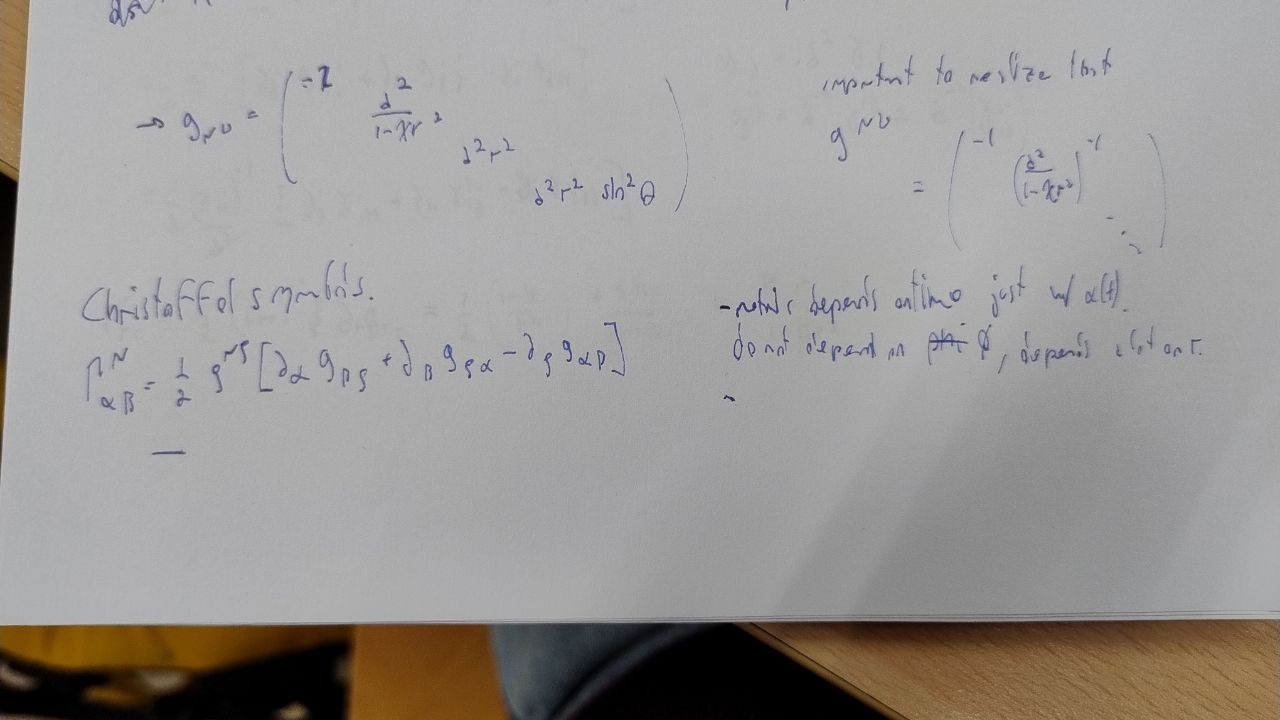
\includegraphics[width=\linewidth]{imm/lec23_2_1.jpg}
\caption{}
\label{imm:lec23_2_1.jpg}
\end{figure}
\begin{figure}[h]
\centering
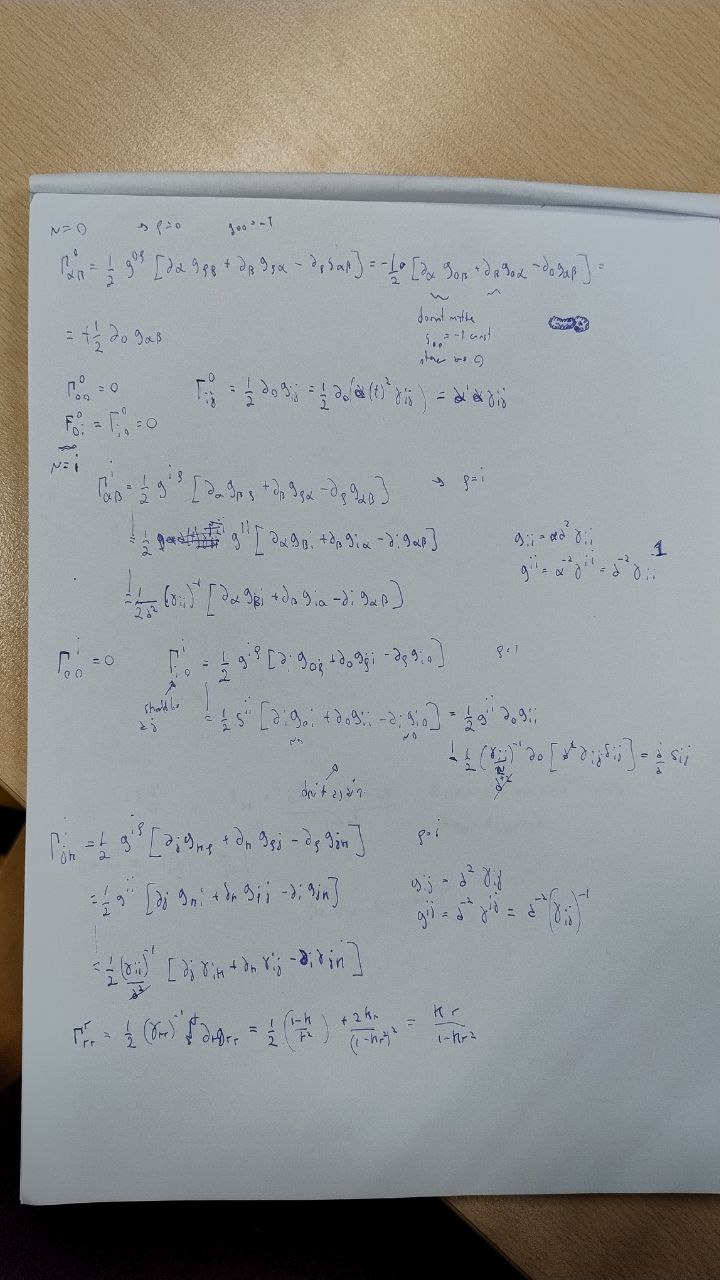
\includegraphics[width=\linewidth]{imm/lec23_2_2.jpg}
\caption{}
\label{imm:lec23_2_2.jpg}
\end{figure}
\begin{figure}[h]
\centering
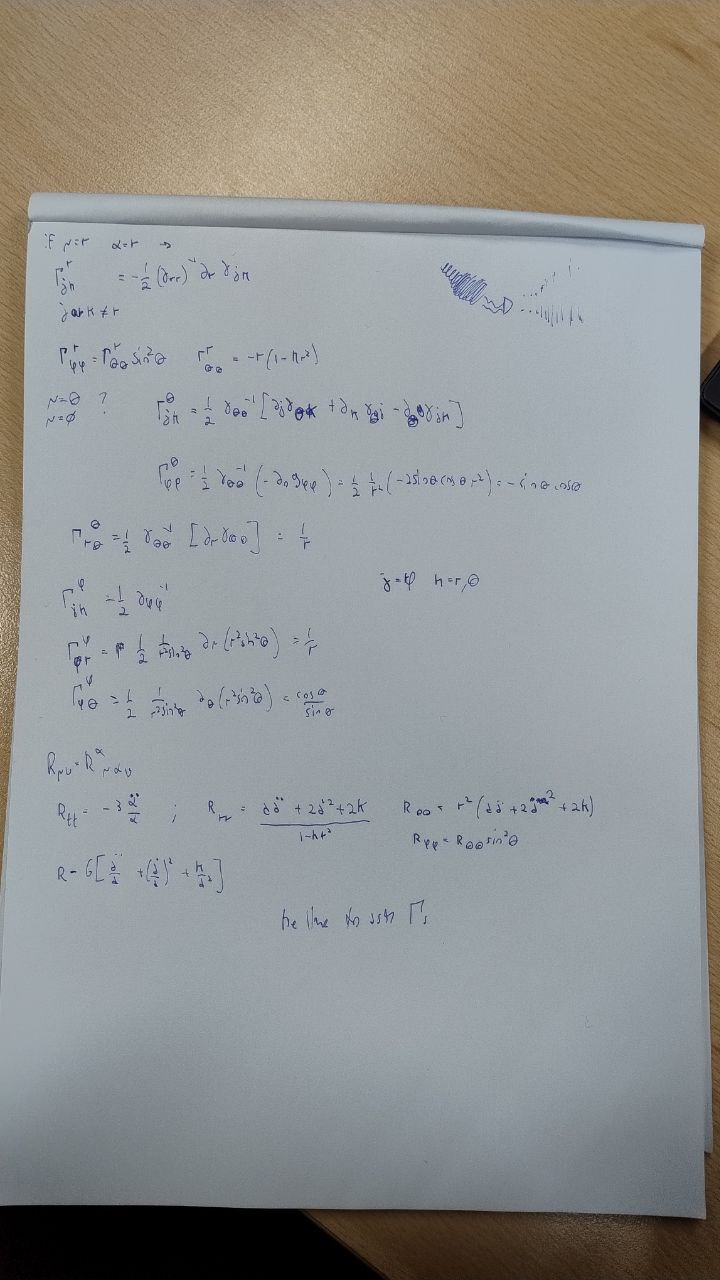
\includegraphics[width=\linewidth]{imm/lec23_2_3.jpg}
\caption{}
\label{imm:lec23_2_3.jpg}
\end{figure}













